\section{QCD in the Continuum}
\subsection{The QCD Lagrangian}
We begin by defining the QCD Lagrangian~\cite{Fritzsch:1973pi} in Euclidean spacetime in terms of quark fields and gluon fields, and discuss the various transformation properties of those fields and the QCD action. As we will see, the advantage of working in Euclidean spacetime is that oscillating exponentials in time become decaying exponentials. This allows us to interpret the Boltzmann factor $e^{-S}$ (where $S$ is the action in Euclidean spacetime) as a probability distribution, allowing us to use Monte Carlo integration to evaluate path integrals in quantum field theory. Additionally, we will see that this gives us access to the low-lying energy spectrum of a theory by allowing us to fit two-point correlation functions to real decaying exponentials. The QCD Lagrangian $\mathcal L_{\rm{QCD}}$ can be written in terms of the fermionic part $\mathcal L_{\rm F}$ and pure-gluon part $\mathcal L_{\rm G}$. In a free theory (i.e.\ without gluons), the fermionic Lagrangian is
\begin{equation}\label{eq:free}
    \mathcal L_{\text{F, free}} = \sum_{f} \overline \psi^{(f)}_{\alpha c}\left((\gamma_\mu)_{\alpha\beta} \partial_\mu + \delta_{\alpha\beta}m^{(f)}\right)\psi^{(f)}_{\beta c}(x),
\end{equation}
where a sum over repeated indices is implied. $\psi$ and $\overline \psi$ are quark and anti-quark fields, respectively, and they carry a flavor index $f$, a Dirac spin index $\alpha$, and a color index $c$. $m^{(f)}$ is the bare mass of the fermion with flavor $f$, and $\gamma_\mu$ are the Euclidean analogs to the familiar Minkowski $\gamma$-matrices satisfying the anticommutation relation $\lbrace\gamma_\mu, \gamma_\nu\rbrace=2\delta_{\mu\nu}\mathbbm 1$, where $\mu\in\lbrace 1,2,3,4\rbrace$ is the Euclidean spacetime index. In its non-interacting form, Eq.~(\ref{eq:free}) appears identical to the familiar QED Lagrangian, except with additional indices for color, which do not mix.

In an interacting theory with gluons, the fermionic part of the Lagrangian becomes
\begin{equation}\label{eq:fermion_lagrangian}
    \mathcal L_{\rm F} = \sum_{f} \overline \psi^{(f)}_{\alpha c}\left((\gamma_\mu)_{\alpha\beta} (\delta_{cd}\partial_\mu + i A_{\mu c d}(x)) + \delta_{\alpha\beta}\delta_{cd} m^{(f)}\right)\psi^{(f)}_{\beta d}(x),
\end{equation}
where we have introduced the gluon fields $A_{\mu c d}$, which carry color indices in addition to spacetime indices. The matrices $A_\mu$ are hermitian and traceless in color space. Being matrices, they make QCD a \emph{non-Abelian} gauge theory, as the gluon fields themselves do not commute. The non-Abelian nature of QCD is the main reason why extracting the low-energy physics is difficult. We define the covariant derivative
\begin{equation}
    D_\mu(x) = \partial_\mu + i A_\mu(x)
\end{equation}
and the field strength tensor
\begin{equation}
    F_{\mu \nu}(x) = -i[D_\mu(x), D_\nu(x)] = \partial_\mu A_\nu(x) - \partial_\nu A_\mu(x) + i[A_\mu(x), A_\nu(x)].
\end{equation}
The gauge fields $A_\mu(x)$ are traceless and hermitian and belong to the Lie algebra $\mathfrak{su}$(3). Therefore, we can write $A_\mu$ in terms of the 8 generators of SU(3), denoted by $T_i$, which form a basis for $\mathfrak{su}$(3), as
\begin{equation}
    A_{\mu}(x)=\sum_{i=1}^{8} A_{\mu}^{(i)}(x) T_{i}.
\end{equation}
We call $A_{\mu}^{(i)}(x)$ the \emph{color components} of the gauge field, and they are real-valued. The generators satisfy the following properties in addition to being traceless, complex, and hermitian:
\begin{equation}
    \tr \left[T_{j} T_{k}\right]=\frac{1}{2} \delta_{j k}
\end{equation}
and
\begin{equation}
    \left[T_{j}, T_{k}\right]=\mathrm{i} f_{j k l} T_{l},
\end{equation}
where $f_{jkl}$ are known as the \emph{structure constants} and are completely anti-symmetric. Conventionally, we choose to represent $\mathfrak{su}$(3) using $T_a = \frac{\lambda_a}{2}$, where $\lambda_a$ are the Gell-Mann matrices~\cite{GellMann:1962xb}.

Now we write down the gluonic part of the QCD Lagrangian,
\begin{equation}\label{eq:Lg}
    \mathcal L_{\rm G} = \frac{1}{2g^2} \tr[F_{\mu\nu}(x) F_{\mu\nu}(x)],
\end{equation}
where $g$ is the QCD coupling parameter. Using the decomposition of the gluon fields into their color components, we can similarly decompose the field strength tensor into its color components to gain more insight into the gluonic part of the Lagrangian:
\begin{equation}
    \begin{aligned}
        F_{\mu \nu}(x) &=\sum_{i=1}^{B} F_{\mu \nu}^{(i)}(x) T_{i}, \\
        F_{\mu \nu}^{(i)}(x) &=\partial_{\mu} A_{\nu}^{(i)}(x)-\partial_{\nu} A_{\mu}^{(i)}(x)-f_{i j k} A_{\mu}^{(j)}(x) A_{\nu}^{(k)}(x).
        \end{aligned}
\end{equation}
Plugging this into Eq.~(\ref{eq:Lg}), we find that the QCD Lagrangian contains 3- and 4-vertex gluonic self-interactions. This makes QCD and QED fundamentally different: in QED we have linear superposition since the massless vector boson (the photon) does not self-interact, whereas in QCD, linear superposition never applies due to the gluon self-interactions.
\subsection{Transformation Properties of the Quark and Gluon Fields}
QCD is an SU(3) gauge theory, meaning the action is invariant under local SU(3) gauge transformations of the quark and gluon fields. Such a gauge transformation can be associated with a $3\times3$ unitary color-space transformation $\Omega(x)$ at each spacetime point $x$, which also has the property $\det[\Omega(x)] = 1$. In order to ensure gauge invariance, we demand that the quark fields transform as
\begin{equation}\label{eq:quark_transf}
    \begin{aligned}
    \psi(x) &\rightarrow \psi^{\prime}(x)=\Omega(x) \psi(x)\\
    \overline{\psi}(x) &\rightarrow \overline{\psi}^{\prime}(x)=\overline{\psi}(x) \Omega(x)^{\dagger},
    \end{aligned}
\end{equation}
and the gluon fields transform as
\begin{equation}\label{eq:gluon_transf}
    A_{\mu}(x) \rightarrow A_{\mu}^{\prime}(x)=\Omega(x) A_{\mu}(x) \Omega(x)^{\dagger}+\mathrm{i}\left(\partial_{\mu} \Omega(x)\right) \Omega(x)^{\dagger},
\end{equation}
where we have suppressed Dirac indices and used matrix/vector notation for the color indices. One can then verify that Eqs.~(\ref{eq:quark_transf}) and (\ref{eq:gluon_transf}) leave the action $S=\int d^4 x \lbrace \mathcal L_{\rm{F}} + \mathcal L_{\rm{G}}\rbrace$ invariant.
\section{Discretizing QCD on the Lattice}
To facilitate our nonperturbative computations, we must formulate QCD on a spacetime lattice. We consider our lattice $\Lambda$ as an isotropic four-dimensional grid of points, indexed by a 4-tuple of integers $n$ such that $x=an$, where $a$ is the lattice spacing. That is, we can write
\begin{equation}
    \Lambda = \lbrace n = (n_1, n_2, n_3, n_4)\rbrace,
\end{equation}
where $n_i$ are integers. We will later also consider anisotropic lattices. Since a lattice has finite spacing, that implies a momentum cutoff, which also acts as an ultraviolet regulator for the theory. That is, the $i$ component momentum is restricted to $p_i \in (-\frac{\pi}{a}, \frac{\pi}{a}]$. Additionally, we will work with periodic boundary conditions, which discretizes the momentum $\bs p = \frac{2\pi \bs n}{L}$, where $\bs n$ is a vector of integers and $L$ is the length of the lattice. 
\subsection{Free Fermions}
We begin with a naive approach to discretizing fermions on the lattice, which will then be improved upon. The continuum action for one free fermion with a bare mass $m$ can be written as
\begin{equation}\label{eq:action_ff}
    S_{F}^{0}[\psi, \overline{\psi}]=\int d^{4} x \; \overline{\psi}(x)\left(\gamma_{\mu} \partial_{\mu}+m\right) \psi(x).
\end{equation}
A first pass at discretizing Eq.~(\ref{eq:action_ff}) involves replacing the integral by a sum, replacing $x$ by $n$, and rewriting the derivative terms as simple finite differences, like so,
\begin{gather}
    \int d^4x \rightarrow a^4 \sum_n \\
    \psi(x) \rightarrow \psi(n) \\
    \overline\psi(x) \rightarrow \overline\psi(n) \\
    \partial_{\mu} \psi(x) \rightarrow \frac{1}{2 a}(\psi(n+\hat{\mu})-\psi(n-\hat{\mu})).
\end{gather}
We immediately find that such a discretization scheme breaks local SU(3) gauge invariance, due to terms of the form $\overline\psi(n) \psi(n+\hat\mu)$.
\subsection{Gauge Fields and Link Variables}
Though we expect that gauge invariance for the free fermion action is restored in the limit $a \rightarrow 0$, we wish to maintain exact gauge invariance for finite $a$ in the entire discretized action. In determining how to discretize the gluon fields, we are guided by this requirement. Under a local gauge transformation $\Omega(n)$,
\begin{equation}
    \overline{\psi}(n) \psi(n+\hat{\mu}) \rightarrow \overline{\psi}(n) \Omega(n)^{\dagger} \Omega(n+\hat{\mu}) \psi(n+\hat{\mu}),
\end{equation}
which is obviously not gauge-invariant. We can fix this issue by introducing new fields $U_\mu(n)$, called \emph{link variables}~\cite{Wilson:1974sk}, which transform under a gauge transformation as
\begin{equation}\label{eq:link_transf}
    U_{\mu}(n) \rightarrow \Omega(n) U_{\mu}(n) \Omega(n+\hat{\mu})^{\dagger}.
\end{equation}
These link variables are matrix-valued, and are elements of the gauge group SU(3). They are also directionally oriented, and are defined such that $U_{-\mu}(n) \equiv U_{\mu}(n-\hat{\mu})^{\dagger}$. They can be visually represented as living on the links between lattice sites, as depicted in Fig.~\ref{fig:links}.
\begin{figure}
    \centering
    % 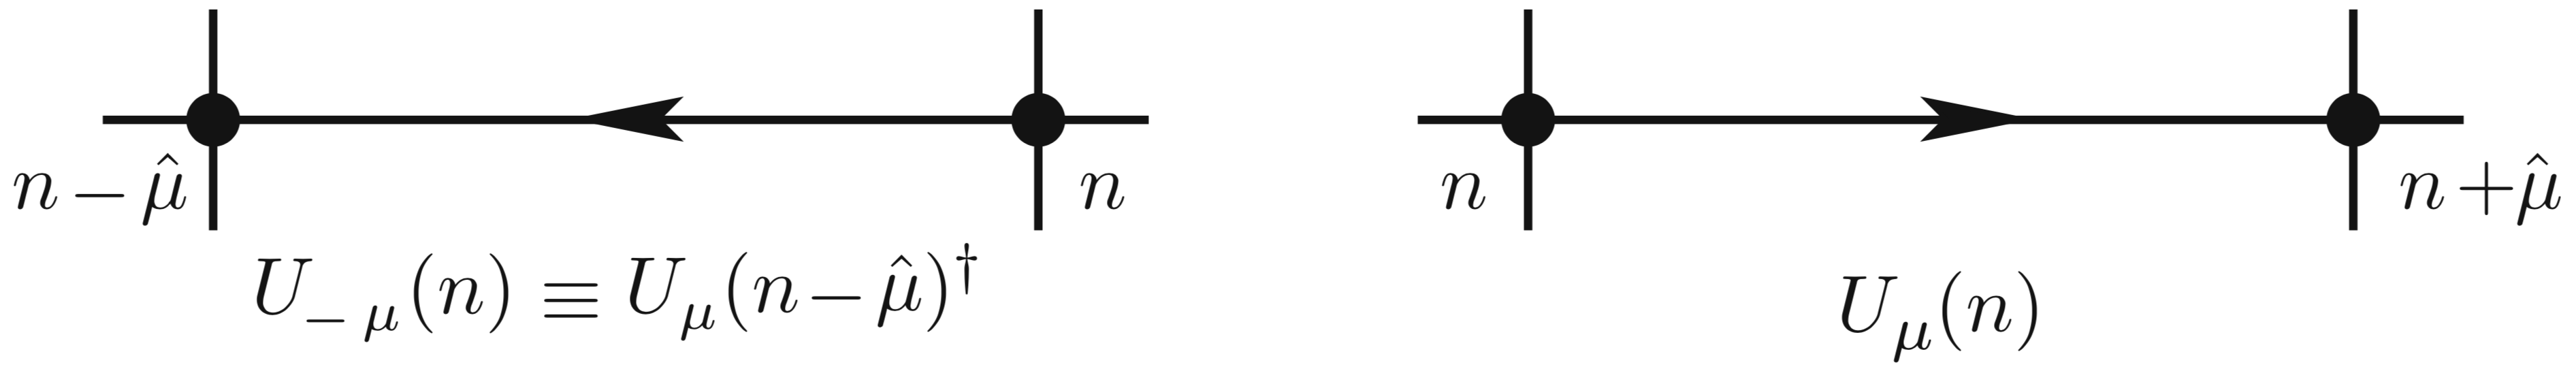
\includegraphics[scale=0.2]{figures/links.png}
    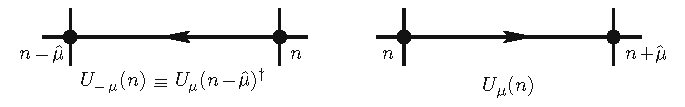
\includegraphics[width=0.7\textwidth]{figures/links.pdf}
    \caption{Link variables, depicted as linking two adjacent lattice sites.}
    \label{fig:links}
\end{figure}
We then propose the following form for the naively discretized interacting fermionic action for one flavor as follows, which one can verify to be gauge-invariant:
\begin{equation}\label{eq:lattice_fermion_action}
    S_{F}[\psi, \overline{\psi}, U]=a^{4} \sum_{n \in A} \overline{\psi}(n)\left(\sum_{\nu=1}^{4} \gamma_{\mu} \frac{U_{\mu}(n) \psi(n+\hat{\mu})-U_{-\mu}(n) \psi(n-\hat{\mu})}{2 a}+m \psi(n)\right).
\end{equation}
In taking the limit $a\rightarrow 0$, the fermionic action will contain $\mathcal O(a)$ lattice artifacts. Now that we have identified a candidate for a gauge-invariant discretized interacting fermion action, it remains to relate the link variables $U_\mu(n)$ to the continuum gauge fields $A_\mu(x)$. In the continuum, there is an object which satisfies the same gauge transformation properties as the link variables (see Eq.~(\ref{eq:link_transf})), and that object is the gauge transporter,
\begin{equation}
    G(x, y)=P \exp \left(\mathrm{i} \int_{\mathcal{C}_{x y}} A \cdot d s\right),
\end{equation}
where $C_{xy}$ is a curve connecting two points $x$ and $y$, and $P$ denotes path-ordering. The link variables approximate this gauge transporter, i.e.\ $U_\mu(n) = G(n, n+\hat \mu) + \mathcal O(a)$, and are given by
\begin{equation}
    U_{\mu}(n)=\exp \left(\mathrm{i} a A_{\mu}(n)\right).
\end{equation}
One can verify that in the continuum limit $a\rightarrow 0$, the action in Eq.~(\ref{eq:lattice_fermion_action}) reduces to its continuum form given by integrating the Lagrangian in Eq.~(\ref{eq:fermion_lagrangian}). Note that we have gone from using $\mathfrak{su}(3)$ Lie algebra-valued fields $A_\mu(x)$ to variables $U_\mu(x)$ which are elements of the Lie group SU(3). This will become relevant in defining the path integral on the lattice.
\subsection{Fermion Doubling}
We define the \emph{Dirac Matrix} $M[U]$ for a theory with one fermion flavor by rewriting the fermion action in Eq.~(\ref{eq:lattice_fermion_action}) as
\begin{equation}
    S_F[\psi, \overline \psi, U] = \sum_{n,m\in \Lambda} \sum_{a,b,\alpha,\beta} \overline \psi(n)_{\alpha a} M(n|m)_{\alpha\beta;a b} \psi(m)_{\beta b},
\end{equation}
implying that
\begin{equation}
    M(n | m)_{\alpha \beta; a b} = a^4\sum_{\mu=1}^{4}\left(\gamma_{\mu}\right)_{\alpha \beta} \frac{U_{\mu}(n)_{a b} \delta_{n+\hat{\mu}, m}-U_{-\mu}(n)_{a b} \delta_{n-\hat{\mu}, m}}{2 a}+m \delta_{\alpha \beta} \delta_{a b} \delta_{ m}.
\end{equation}
The free quark propagator on the lattice is found by inverting the Dirac matrix when the gauge fields are set to $U_\mu(n) = \mathbbm 1$. In momentum space, the Dirac matrix is given by
\begin{equation}\label{eq:ms_dirac}
    \widetilde{M}(p)=a^4 \left(m + i \sum_{\mu=1}^{4} \gamma_{\mu} \frac{\sin \left(p_{\mu} a\right)}{a}\right)
\end{equation}
and its inverse is
\begin{equation}
    \widetilde M^{-1}(n|m) = a^{-4}\frac{m - ia^{-1}\sum_\mu \gamma_\mu \sin(p_\mu a)}{m^2 + a^{-2}\sum_\mu\sin(p_\mu a)^2}.
\end{equation}
If we examine this propagator in the massless case, $m=0$, we find a pole at $p^2 = 0$, as we would expect. However, we also find 15 additional poles at the corners of the first Brillouin zone, i.e.\ at $p=(\pi / a, 0,0,0),(0, \pi / a, 0,0), \ldots,(\pi / a, \pi / a, \pi / a, \pi / a)$. These extra poles are known as the \emph{doublers}. They are not present in the continuum (just take $a\rightarrow 0$ in the denominator of the propagator to see this), but on the lattice, we must deal with these unphysical poles. Wilson found a clever way to deal with these doublers~\cite{Wilson:1975id} by adding an additional term, now known as the \emph{Wilson term}, to the Dirac matrix. In momentum space, the Dirac matrix with the added Wilson term is (c.f. Eq.~(\ref{eq:ms_dirac}))
\begin{equation}
    \widetilde{M}(p)=a^4\left(m +i \sum_{\mu=1}^{4} \gamma_{\mu} \frac{\sin \left(p_{\mu} a\right)}{a}+ \sum_{\mu=1}^{4}\frac{\left(1-\cos \left(p_{\mu} a\right)\right)}{a}\right).
\end{equation}
The Wilson term vanishes at $p=(0,0,0,0)$, but acts as an extra mass term at each corner of the Brillioun zone. These mass terms scale as $\frac{1}{a}$, so for small lattices, they will decouple from the theory and not affect the low energy spectrum. Inverting the Fourier transform, the Wilson term turns out to be a discretization of $-\frac{a}{2}\partial_\mu \partial_\mu$, which vanishes in the continuum limit.

While the Wilson term solves our fermion doubling problem, it introduces a new problem. Since the Wilson term is proportional to $\mathbbm 1$ in Dirac space, it does not anticommute with $\gamma_5 = \gamma_4 \gamma_1 \gamma_2 \gamma_3$, which implies that it violates chiral symmetry. (See Section 7.2 in Ref.~\cite{Gattringer:2010zz} for more details.) This problem of chiral symmetry breaking is not a defect of only Wilson's solution to fermion doubling, but of any solution that attempts to add terms to free the theory of doublers, as shown in the famous ``no-go'' theorem of Nielson and Ninomiya~\cite{Nielsen:1981hk}.
\subsection{The Wilson Gauge Action}
After constructing a discretized version of the fermion action, it remains to construct a discretized version of the gauge action. The first step is to identify a gauge-invariant object constructed only of link variables. An ordered product of link variables
\begin{equation}
    P[U]=U_{\mu_{0}}\left(n_{0}\right) U_{\mu_{1}}\left(n_{0}+\hat{\mu}_{0}\right) \ldots U_{\mu_{k-1}}\left(n_{1}-\hat{\mu}_{k-1}\right) \equiv \prod_{(n, \mu) \in \mathcal{P}} U_{\mu}(n)
\end{equation}
along a path $\mathcal P$ on the lattice is the lattice analog to the continuum gauge transporter. This product shares the same transformation properties as the link variables and the continuum gauge transporter, i.e.\
\begin{equation}
    P[U] \rightarrow \Omega\left(n_{0}\right) P[U] \Omega\left(n_{1}\right)^{\dagger}.
\end{equation}
If we choose a path that forms a closed loop $\mathcal L$, then such a product transforms under a gauge transformation as
\begin{equation}\label{eq:loop}
    \prod_{(n, \mu) \in \mathcal{L}} U_{\mu}(n) \rightarrow \Omega\left(n_{0}\right) \prod_{(n, \mu) \in \mathcal{L}} U_{\mu}(n) \Omega\left(n_{0}\right)^{\dagger},
\end{equation}
since the color rotations $\Omega(n)$ cancel out at every intermediate point due to unitary. We can then use the cyclicity of the trace to form a gauge-invariant object out of Eq.~(\ref{eq:loop}). Hence,
\begin{equation}
    \tr[\prod_{(n, \mu) \in \mathcal{L}} U_{\mu}(n)]
\end{equation}
is gauge-invariant. The shortest closed loop is called the \emph{plaquette}, which is defined as a product of four link variables,
\begin{equation}
    U_{\mu \nu}(n)=U_{\mu}(n) U_{\nu}(n+\hat{\mu}) U_{-\mu}(n+\hat{\mu}+\hat{\nu}) U_{-\nu}(n+\hat{\nu}).
\end{equation}
With these definitions, we now write down Wilson's formulation of the gauge action on the lattice, which is a sum over all possible plaquettes on the lattice (only counting one orientation for each plaquette):
\begin{equation}
    S_{G}[U]=\frac{2}{g^{2}} \sum_{n \in \Lambda} \sum_{\mu<\nu} \operatorname{Re}\,\operatorname{tr}\left[\mathbbm{1}-U_{\mu \nu}(n)\right].
\end{equation}
In the continuum limit $a\rightarrow 0$, it can be shown that this reduces to the continuum version given by integrating the Lagrangian in Eq.~(\ref{eq:Lg}). In taking the limit, the action will contain $\mathcal O(a^2)$ lattice artifacts, that is,
\begin{equation}
    S_{G}[U]=\frac{2}{g^{2}} \sum_{n \in \Lambda} \sum_{\mu<\nu} \operatorname{Re} \operatorname{tr}\left[\mathbbm{1}-U_{\mu \nu}(n)\right]=\frac{a^{4}}{2 g^{2}} \sum_{n \in A} \sum_{\mu, \nu} \operatorname{tr}\left[F_{\mu \nu}(n)^{2}\right]+\mathcal{O}\left(a^{2}\right).
\end{equation}
The Wilson action is just one way to formulate a discretized gauge action. We will discuss different discretization strategies in order to reduce the discretization error to higher orders in $a$.
\subsection{Improving the Discretized Action}\label{sec:improved_action}
In our naively discretized theory, the fermionic action action contains $\mathcal O(a)$ lattice artifacts and the gauge action contains $\mathcal O(a^2)$ artifacts. By adding terms to the action which cancel these artifacts but which vanish in the continuum limit, we can improve discretization errors to higher orders in $a$. This is called \emph{Symanzik improvement}~\cite{Symanzik:1983dc}. For example, we make use of a \emph{clover improved}~\cite{Sheikholeslami:1985ij} action, which involves adding a term to the Wilson action,
\begin{equation}
    c_{\mathrm{sw}} a^{5} \sum_{n \in \Lambda} \sum_{\mu<\nu} \bar{\psi}(n) \frac{1}{2} \sigma_{\mu \nu} \widehat{F}_{\mu \nu}(n) \psi(n),
\end{equation}
where $c_{\mathrm{sw}}$ is a real coefficient, called the Sheikholeslami–Wohlert coefficient,
\begin{equation}
    \widehat{F}_{\mu \nu}(n)=\frac{-\mathrm{i}}{8 a^{2}}\left(Q_{\mu \nu}(n)-Q_{\nu \mu}(n)\right),
\end{equation}
\begin{equation}
    \sigma_{\mu \nu} \equiv\left[\gamma_{\mu}, \gamma_{\nu}\right] / 2 \mathrm{i},
\end{equation}
and
\begin{equation}
    Q_{\mu \nu}(n) \equiv U_{\mu, \nu}(n)+U_{\nu,-\mu}(n)+U_{-\mu,-\nu}(n)+U_{-\nu, \mu}(n).
\end{equation}
The clover term is named as such because it is constructed from four adjacent plaquettes, as depicted in Fig.~\ref{fig:clover}.
\begin{figure}
    \centering
    % 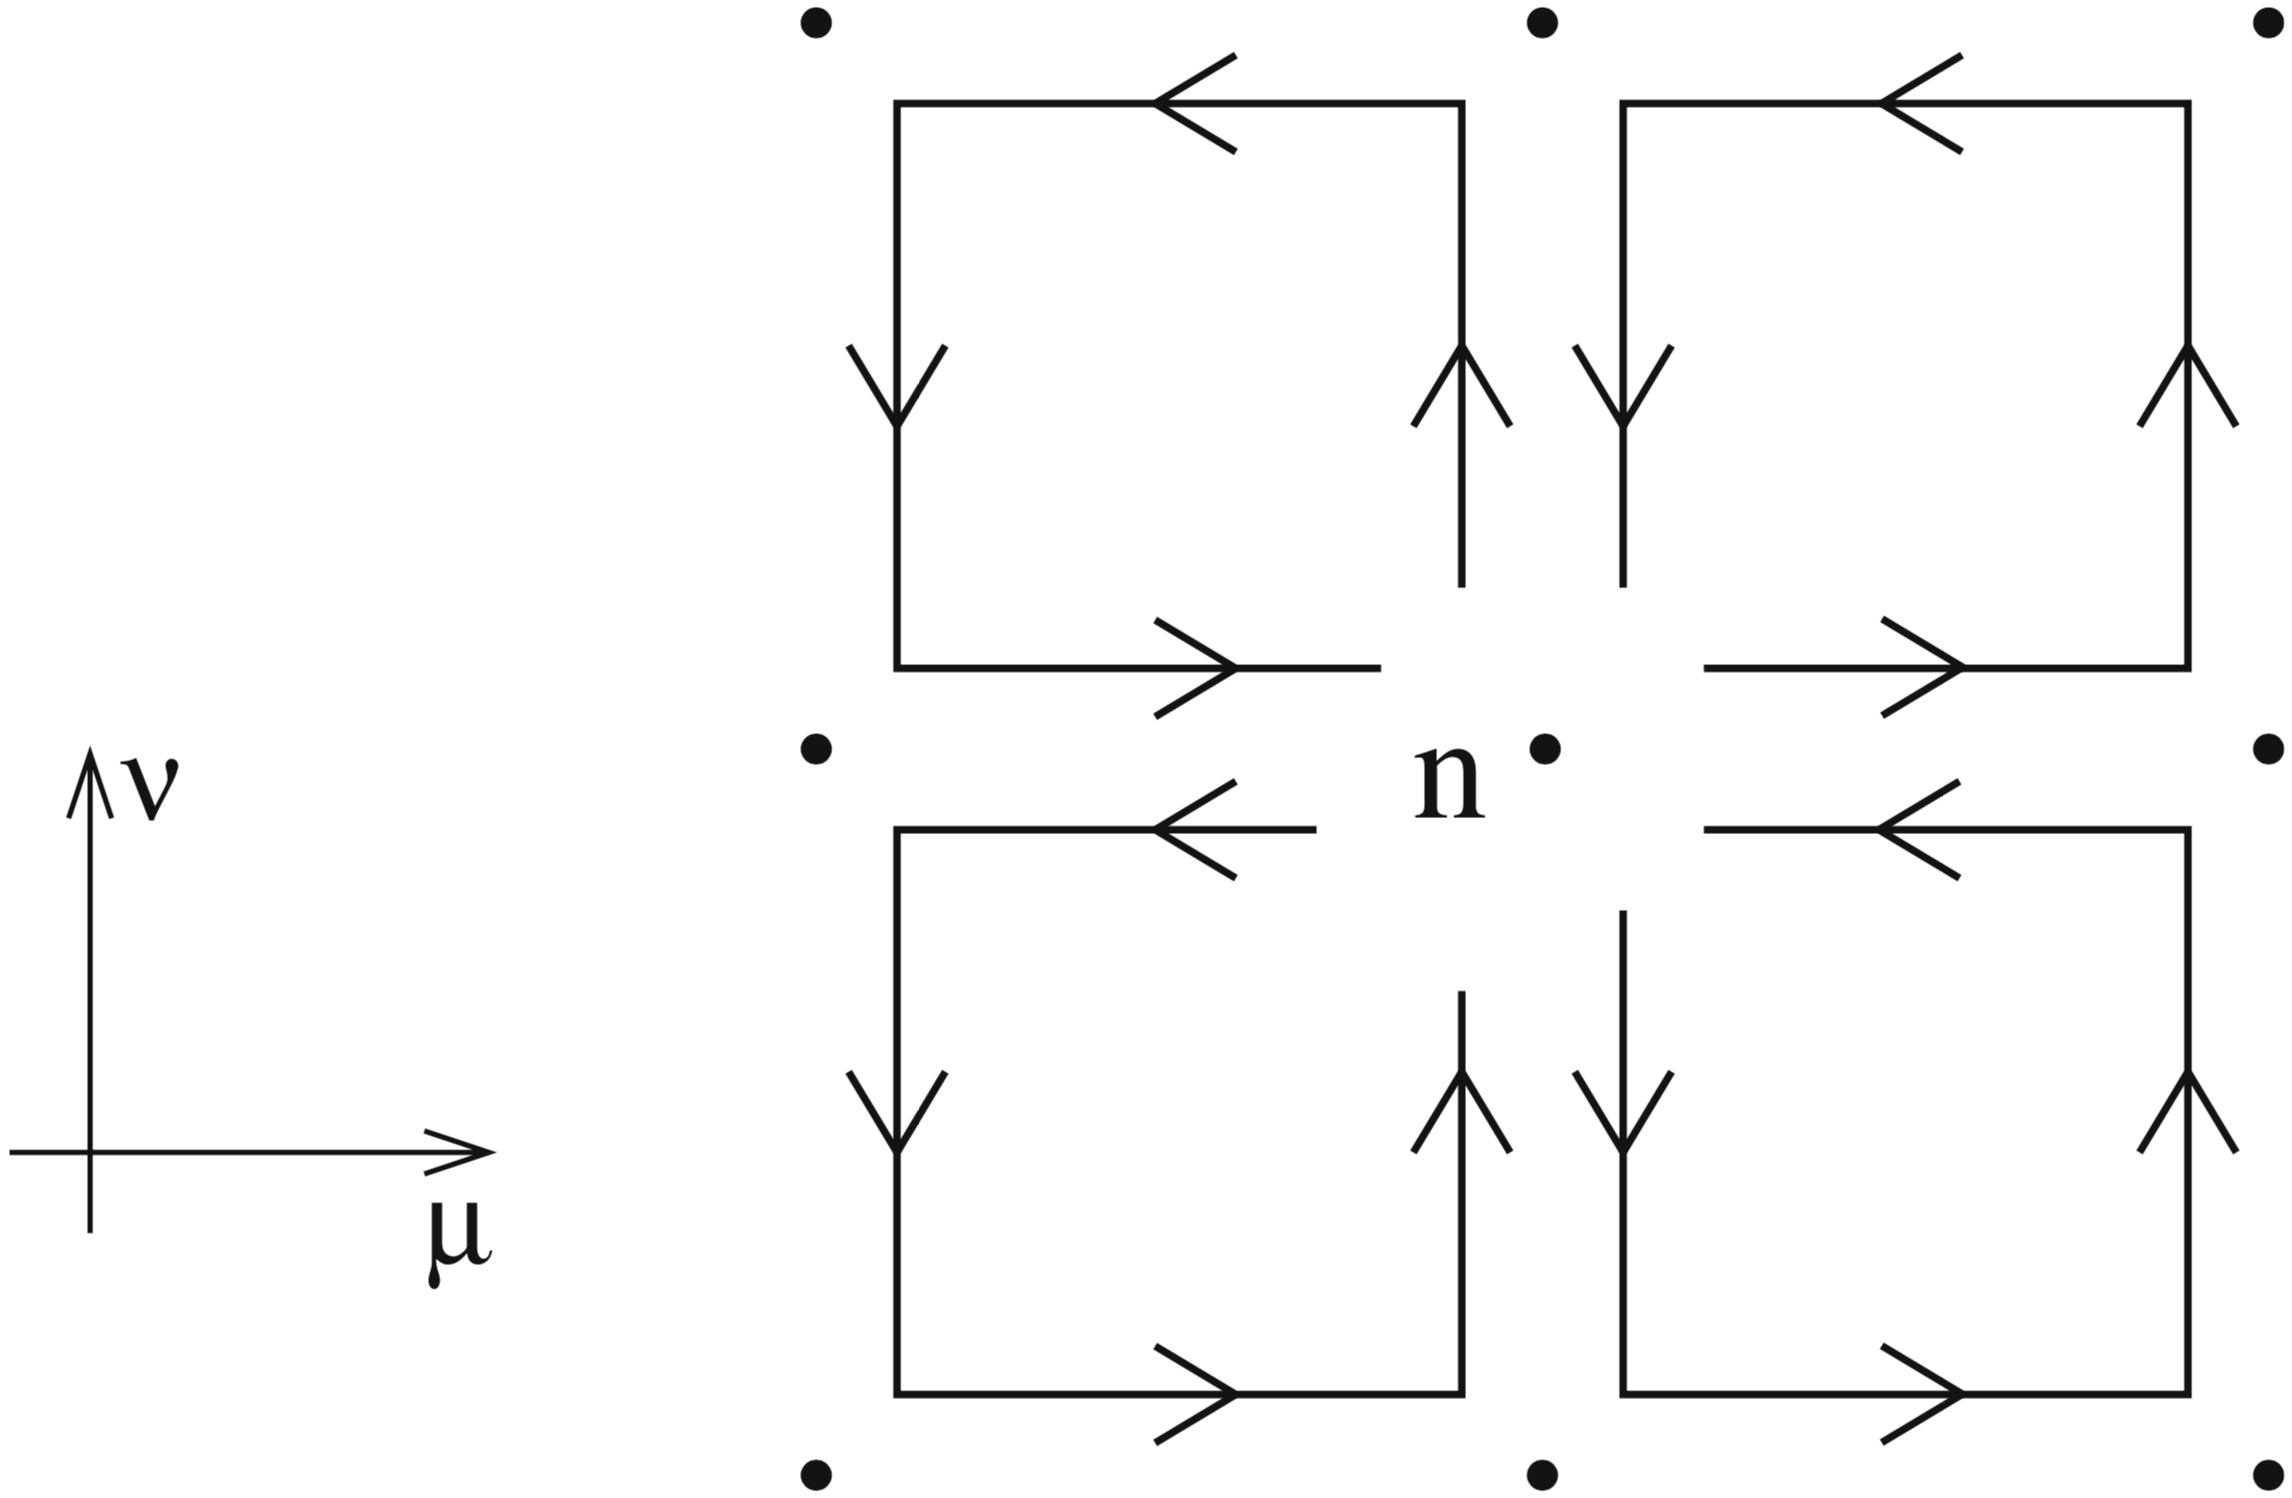
\includegraphics[scale=0.2]{figures/clover.png}
    \hspace*{-1in}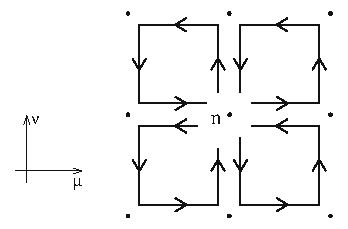
\includegraphics[width=0.6\textwidth]{figures/clover.pdf}
    \caption{Depiction of the clover term, built out of four plauqettes.}
    \label{fig:clover}
\end{figure}

In addition to Symanzik improvements, there are so-called \emph{tadpole} improvements~\cite{Lepage:1992xa} that can be made to the gauge action. These seek to correct contributions from QCD tadpole diagrams that appear at low energy, when the coupling is large. For a small coupling $g$, we may reasonably expand the link variables as $U_{\mu}(x) \equiv e^{i a g A_{\mu}(x)} \rightarrow 1+i a g A_{\mu}(x)$. It turns out, however, that higher order terms are suppressed by powers of $g^2$, and so when the coupling is large, there will be contributions from QCD tadpoles. For a detailed presentation, see~\cite{Lepage:1992xa}. In order to deal with these tadpoles, we rescale the link variables as $U \rightarrow \frac{U}{u}$, where
\begin{equation}
    u=\left\langle\frac{1}{3} \operatorname{Re} \operatorname{Tr} U_{\mu \nu}\right\rangle^{1 / 4}.
\end{equation}
$u$ is both a parameter of the action and an observable, so we must iteratively tune $u$ in the action such that the $u$ we observe is the same as the $u$ we put into the action.

In practice, our lattices are anisotropic~\cite{Edwards:2008ja, Lin:2008pr}. The motivation for this is that the primary observables we measure are temporal correlators whose signal-to-noise ratios decrease as time separation increases. To combat this issue, we could use a finer lattice in order to sample the correlators at more time separations. The computational cost of refining the lattice in every direction is large, however, so we choose to refine only the temporal direction. That is, we choose an anisotropy $\xi \equiv \frac{a_s}{a_t} > 1$, where $a_s$ is the spatial lattice spacing and $a_t$ is the temporal lattice spacing. $\xi$ is in fact a quantity that undergoes renormalization, so the anisotropy enters into the gauge action as a parameter $\gamma_g$ and into the fermionic action as a parameter $\gamma_f$. Both of these parameters must be tuned to produce the desired renormalized anisotropy.

Finally, we write down the action we use in this work. The gauge action is a Symanzik-improved L\"uscher-Weisz action~\cite{Luscher:1984xn,Luscher:1985zq}, and uses tadpole improvement coefficients from~\cite{Morningstar:1997ff, Morningstar:1999rf, Lin:2008pr,Edwards:2008ja}:
\begin{equation}
    S_{G}^{\xi}[U]=\frac{\beta}{3 \gamma_{g}}\left[\sum_{x, i \neq j}\left(\frac{5}{6 u_{s}^{4}} \Omega_{\mathcal{P}_{i j}}(x)-\frac{1}{12 u_{s}^{6}} \Omega_{\mathcal{R}_{i j}}(x)\right)+\sum_{x, i}\left(\frac{4}{3 u_{s}^{2} u_{t}^{2}} \Omega_{\mathcal{P}_{i t}}(x)-\frac{1}{12 u_{s}^{4} u_{t}^{2}} \Omega_{\mathcal{R}_{i t}}\right)\right].
\end{equation}
Here, $P$ is a plaquette, $\Omega_P = \Re \Tr(1-P)$, $R$ is a $2\times 1$ planar Wilson loop, $u_s$ and $u_t$ are the aforementioned tadpole improvement coefficients, $\beta$ is the inverse gauge coupling, and $\gamma_g$ is the bare anisotropy parameter for the gauge sector. Notice that only improvements in spatial links have been included. Lattice gauge-field actions which involve more than two time slices often lead to temporal correlators which do not fall exponentially in a simple way. This action has $\mathcal O(a_s^4, a_t^2, g^2a_s^2)$ discretization errors. The fermionic part of the action is given by
\begin{equation}
    \begin{aligned}
        S_{F}^{\xi}[U, \bar{\psi}, \psi] &=\sum_{x} \overline{\hat{\psi}}(x) \frac{1}{\tilde{u}_{t}}\left\{\tilde{u}_{t} \hat{m}_{0}+\gamma_{t} \hat{W}_{t}+\frac{1}{\gamma_{f}} \sum_{s} \gamma_{s} \hat{W}_{s}\right.\\
        &\left.-\frac{1}{2}\left[\frac{1}{2}\left(\frac{\gamma_{g}}{\gamma_{f}}+\frac{1}{\xi}\right) \frac{1}{\tilde{u}_{t} \tilde{u}_{s}^{2}} \sum_{s} \sigma_{t s} \hat{F}_{t s}+\frac{1}{\gamma_{f}} \frac{1}{\tilde{u}_{s}^{3}} \sum_{s<s^{\prime}} \sigma_{s s^{\prime}} \hat{F}_{s s^{\prime}}\right]\right\} \hat{\psi}(x).
        \end{aligned}
\end{equation}
Here, $\gamma_f$ is the bare anisotropy for the gauge sector, $\xi = \frac{a_s}{a_t}$ is the renormalized anisotropy, $\gamma_\mu$ and $\sigma_{\mu\nu} = \frac{1}{2}[\gamma_\mu, \gamma_\nu]$ are Dirac gamma matrices, $\tilde u_s$ is the spatial tadpole improvement factor, and $\tilde u_t$ is the temporal tadpole improvement factor. Hats denote dimensionless quantities that relate to dimensionful quantities by scaling with appropriate factors of the lattice spacing. $\hat{\psi}=a_{s}^{3 / 2} \psi$ where $\psi$ is the quark field, $\hat{m}_{0}=m_{0} a_{t}$ where $m_0$ is the bare quark mass, and $\hat{F}_{\mu \nu}=a_{\mu} a_{\nu} F_{\mu \nu}=\frac{1}{4} \operatorname{Im}\left(\mathcal{P}_{\mu \nu}(x)\right)$ where $F_{\mu\nu}$ is the field strength tensor. $\hat W$ is the \emph{Wilson operator}, and is given by
\begin{equation}
    \hat{W}_{\mu} \equiv \hat{\nabla}_{\mu}-\frac{1}{2} \gamma_{\mu} \hat{\Delta}_{\mu},
\end{equation}
where
\begin{equation}
    \hat{\nabla}_{\mu}=a_{\mu} \nabla_{\mu},\; \hat{\Delta}_{\mu}=a_{\mu}^{2} \Delta_{\mu}.
\end{equation}
This action has $\mathcal{O}\left(g^{2} a_{s}, g^{2} a_{t}, a_{s}^{2}, a_{t}^{2}\right)$ discretization errors. It is also important to mention that the link variables in the fermionic action are \emph{stout-smeared}~\cite{Morningstar:2003gk}, which we will discuss further in Chapter~\ref{ch:operators}. The use of smeared link variables in the action leads to better chiral behavior.
\subsection{Parameter Tuning}\label{sec:tuning}
\subsubsection{Anisotropy}
The parameters we put into our action are bare parameters. We obtain these parameters by choosing a set of observables, and tuning the bare parameters in our action such that their desired values are produced. For example, we desire a renormalized anisotropy $\xi\approx 3.5$, and must tune the values $\gamma_g$ and $\gamma_f$ to obtain this. In order to tune $\gamma_g$, we measure the following quantities~\cite{Klassen:1998ua}:
\begin{equation}
    \begin{aligned}
        R_{s s}(x, y)&=\frac{W_{s s}(x, y)}{W_{s s}(x+1, y)},\\
        R_{s t}(x, t)&=\frac{W_{s t}(x, t)}{W_{s t}(x+1, t)},
    \end{aligned}
\end{equation}
where $W_{\mu\nu}(x_\mu, x_\nu)$ is the expectation value of a Wilson loop of size $x_\mu$ and $x_\nu$ and oriented in the $\mu$ and $\nu$ directions, and then demand that $R_{s s}(x, y)=R_{s t}(x, \xi t)$.  In order to tune $\gamma_f$, we impose a continuum dispersion relation for mesons on the lattice,
\begin{equation}
    a_{t}^{2} E^{2}(\boldsymbol{p})=a_{t}^{2} m^{2}+\frac{a_{s}^{2} \boldsymbol{p}^{2}}{\xi^{2}}.
\end{equation}
We find that in order to attain $\xi\approx 3.5$, we set $\gamma_g = 4.3$ and $\gamma_f = 3.4$.
\subsubsection{Gauge Coupling and Lattice Spacing}
The renormalization scheme we use requires that the coupling and masses in the lattice QCD action vary (or run) with the ultraviolet cutoff such that observables tend to their physical values as the cutoff is removed. The lattice spacing acts as a cutoff by eliminating very small wavelengths from the theory.  The cutoff is proportional to the inverse lattice spacing, limiting momenta to the first Brillouin zone. We tune the inverse coupling $\beta$ in our action to obtain a desired lattice spacing. Determining the lattice spacing using a physical observable is known as \emph{setting the scale}. One way to set the scale is by choosing a particle, say the $\Omega$, and requiring that its mass measured on the lattice should equal its physical mass. That is, we calculate
\begin{equation}
    a_t = \frac{a_t m}{m_{\rm{Phys}}},
\end{equation}
where $a_t m$ is the quantity we directly measure in a lattice calculation. In our calculations, this yields $a_t\approx 0.034$ fm, giving $a_s\approx 0.12$ fm, and we obtain these values by choosing $\beta = 1.5$.
\subsubsection{Quark Masses}
As we will discuss further in Chapter~\ref{ch:operators}, we work in a theory of $N_f=2+1$ QCD, meaning there are three flavors of quarks, two of which have degenerate masses. These are the degenerate up and down quarks (collectively referred to as the \emph{light} quarks), and the strange quark. An important flaw of our calculations is that we work in a theory of an unphysically heavy pion. This is necessary for two reasons. First, finite volume corrections to the theory are exponentially suppressed by a factor of $e^{-m_\pi L}$, where $m_\pi$ is the mass of the pion (in general, it is the mass of the lightest state in the theory) and $L$ is the spatial extent of the lattice. It is necessary that the \emph{correlation length}, $m_\pi L$ is $>1$, but in practice, a good rule of thumb is to require $m_\pi L > 4$ or so. Second, inverting Dirac matrices (which we will soon see to be an important step of our calculation) becomes much more computationally difficult at lower pion masses, and increases the odds that the Dirac matrices will become ill-conditioned.

In order to tune the light and strange quark masses, we aim to set the following ratios to their physical values~\cite{Lin:2008pr}:
\begin{equation}
        l_{\Omega}=\frac{9 m_{\pi}^{2}}{4 m_{\Omega}^{2}},\quad
        s_{\Omega}=\frac{9\left(m_{K}^{2}-m_{\pi}^{2}\right)}{4 m_{\Omega}^{2}},
\end{equation}
where $m_K$ is the mass of the kaon, $m_\pi$ is the mass of the pion, and $m_\Omega$ is the mass of the $\Omega$ baryon. These ratios are chosen because first-order chiral perturbation theory tells us that they should be proportional to their associated quark masses~\cite{Lin:2008pr}. $s_\Omega$ is set to its physical value, and $l_\Omega$ is lowered to a value 
that is unphysical but allows calculations to remain possible. Using this method of tuning, the bare quark masses are set to be $a_t m_l = -0.0860$ for the light quarks, 
and $a_t m_s = -0.0743$ for the strange quark. With these quark masses, our pion mass is 
approximately 230 MeV.

\section{Extracting Energies from Two-Point Correlation Functions}\label{sec:intro_corr}
In order to do spectroscopy, the main observables we calculate on the lattice are time-ordered two-point correlation functions of the form
\begin{equation}
    C(t) = \bra 0 \mathcal O (t+t_0) \overline{\mathcal O}(t_0) \ket 0,
\end{equation}
where $\ket 0$ is the vacuum state, $\overline{\mathcal O}(t_0)$ is an operator that creates a state out of the vacuum at time $t_0$, and $\mathcal O (t+t_0)$ is an operator that annihilates such a state at a later time $t+t_0$. Let $\ket n$ denote the $n^{\rm{th}}$ energy eigenstate of the theory with energy $E_n$, ordered such that $E_n < E_{n+1}$, and let us shift the energies such that the vacuum energy $E_0 \equiv 0$. Then, using a spectral decomposition and working in the Heisenberg picture in imaginary time $t\rightarrow -it$, we can see
\begin{equation}\label{eq:corr_decomp}
    \begin{aligned}
        C(t) &= \sum_{n=0}^\infty \bra 0 e^{H(t+t_0)} \mathcal O(0) e^{-H(t+t_0)} \ket n \bra n e^{H t_0} \overline{\mathcal O}(0)e^{-H t_0} \ket 0 \\
        &=\sum_{n=0}^\infty e^{E_0(t+t_0)} \bra 0 \mathcal O(0) \ket n e^{-E_n(t+t_0)} e^{E_0 t_0} \bra n \overline{\mathcal O}(0) \ket 0 e^{E_n t_0}\\
        & = \sum_{n=0}^\infty \bra 0 \mathcal O(0) \ket n \bra n \overline{\mathcal O}(0)\ket 0 e^{-E_n t}.
    \end{aligned}
\end{equation}
Here, we have made the assumption that $t \ll T$, where $T$ is the temporal length of the lattice, which is necessary to prevent temporal wrap-around effects. It is now clear that by calculating $C(t)$ on the lattice, we have access to the energy spectrum of the theory. In principle, with infinite statistics, we could fit $C(t)$ to obtain the entire spectrum. In practice, however, we can only reliably extract the lowest non-zero energy in this sum by fitting $C(t)$ to single- or two-exponential functions. As we will discuss further in Chapter~\ref{ch:analysis}, we can circumvent this issue by constructing a \emph{matrix} of correlators
\begin{equation}
    C_{ij}(t) = \bra 0 \mathcal O_i(t+t_0) \overline{\mathcal O}_j(t_0) \ket 0
\end{equation}
and using a variational method to find \emph{principal correlators} $C^{(N)}(t)$ satisfying
\begin{equation}
    C^{(N)}(t) \xrightarrow[t\rightarrow \infty]{} A e^{-E_N t}.
\end{equation}

\section{Monte Carlo Path Integration}
A fundamental equation for calculating observables on the lattice is
\begin{equation}
    \expval{\mathcal O}_T = \frac{1}{Z_T} \int \mathcal D[\psi, \overline \psi, U] \mathcal O[\psi, \overline \psi, U] e^{-S[\psi, \overline \psi, U]},
\end{equation}
where $\mathcal O$ denotes an operator corresponding to a desired observable, $T$ denotes the time extent of the lattice, $S$ denotes the Euclidean action, and $Z_T$ is the partition function, given by
\begin{equation}
    Z_T = \int \mathcal D[\psi, \overline \psi, U] e^{-S[\psi, \overline \psi, U]}.
\end{equation}
It turns out that $\expval{\mathcal O}_T = \bra 0 \mathcal O \ket 0$ only in the $T\rightarrow\infty$ limit, but in practice, $T$ is large enough that $\expval{\mathcal O}_T \approx \bra 0 \mathcal O \ket 0$. In the above equations, we are integrating over all configurations of the quark fields, antiquark fields, and link variables representing the gauge fields. It is important to note that the quark and antiquark fields are treated as independent variables. The action can be decomposed as
\begin{equation}
    S[\psi, \overline \psi, U] = \overline \psi M[U] \psi + S_G[U],
\end{equation}
where $M[U]$ is the Dirac matrix which is a functional of the gauge links, and the gauge action $S_G$ is a functional only of the link variables. Integration over the quark fields can be readily done analytically, as the integrals reduce to Gaussian integrals. Wick's theorem gives
\begin{equation}\label{eq:gauge_int}
    \expval{\mathcal O}_T = \frac{\int \mathcal{D}[U] f\left(M^{-1}[U]\right) \det M[U] e^{-S_{G}[U]}}{\int \mathcal{D}[U] \det M[U] e^{-S_{G}[U]}},
\end{equation}
where $f\left(M^{-1}[U]\right)$ is some function of the inverse of the Dirac matrix, given by the relevant Wick contractions.

While the fermions are integrated out analytically, it is intractable to analytically integrate out the gauge fields. This is where the need for numerical integration arises. Numerically integrating over the gauge fields is nontrivial, however, since the integral in Eq.~(\ref{eq:gauge_int}) is of very high dimension due to the fact that we must integrate over a link variable at every single lattice site. The way to proceed is by use of Monte Carlo integration, which is immune to the so-called curse of dimensionality that precludes other standard numerical methods.

The strategy of Monte Carlo integration proceeds as follows. Consider a very high dimensional integral
\begin{equation}
    I_{f}=\int_{\mathcal{V}} \mathcal{D} U p(U) f(U),
\end{equation}
where $p(U)$ is a probability density over the volume $\mathcal V$, and $f(U)$ is some integrable function of the variables $U$. By factoring out a probability density in the integrand, we ensure much better efficiency in Monte Carlo sampling compared to using uniformly random samples of the integrand, since it allows us to focus on sampling points from the integrand that most contribute to the result of the integral. This technique is called \emph{importance sampling}. If we can randomly sample the variables $U$ with probability density $p(U)$ thereby generating a large ensemble $\{U_1,U_2,...,U_{N_U}\}$ of $N_U$ configuartions, then the integral $I_f$ can be approximated as
\begin{equation}\label{eq:mc_est}
    I_{f} \approx \frac{1}{N_{U}} \sum_{k=1}^{N_{U}} f\left(U_{k}\right),
\end{equation}
by the law of large numbers. For large $N_U$ and independently generated $U_k$, then by the central limit theorem, the standard deviation in the approximation of $I_f$ is given by
\begin{equation}
    \sigma_{I_f} = \sqrt{\frac{V(f(U))}{N_U}},
\end{equation}
where $V(f(U))$ is the variance of $f(U)$ with respect to the probability density $p(U)$. This is where the advantage of working in Euclidean spacetime becomes apparent: the real Boltzmann factor $e^{-S_G[U]}$ functions as a probability distribution (up to a normalization constant). It turns out that it is also necessary to include the fermion determinant $\det M$ in the probability distribution, as including it as a part of the observable itself can lead to large statistical uncertainties due to the very large fluctuations about the mean value.~\cite{Gattringer:2010zz} Including the Dirac matrix determinant and the normalization factor, the probability distribution for calculating observables is
\begin{equation}\label{eq:pU}
    p(U)=\frac{\operatorname{det} M[U] e^{-S_{G}[U]}}{\int \mathcal{D}\left[U^{\prime}\right] \operatorname{det} M\left[U^{\prime}\right] e^{-S_{G}\left[U^{\prime}\right]}}.
\end{equation}
The validity of using $p(U)$ as probability distribution is not obvious, as it requires that $\det M$ is real and positive semi-definite. Fortunately, for an even number of mass-degenerate fermions (an approximation we use for the $u$ and $d$ quarks), this can be shown analytically (see Ref.~\cite{Gattringer:2010zz}, 8.2.1). When we add in a strange quark, there is no such analytic guarantee, but we observe empirically that the mass of the strange quark is high enough that the fermion determinant is always found to be positive.

In order to proceed in generating a set of gauge configurations $\{U_i\}$, we make use of Markov chains. A Markov chain is defined as a stochastic process that generates a sequence of states in which the probability of transitioning from one state to another depends only on the current state of the system~\cite{Morningstar:2007zm}. For us, a state is defined by a gauge field configuration. A certain class of Markov chains (those which are \emph{irreducible} and \emph{aperiodic}) have the property that they tend to a \emph{stationary} distribution provided that they satisfy a condition called \emph{detailed balance} defined by
\begin{equation}
    T(U^\prime \leftarrow U)p(U) = T(U \leftarrow U^\prime)p(U^\prime),
\end{equation}
where $T(U^\prime \leftarrow U)$ is the probability of transitioning to a state $U^\prime$ if the current state is $U$. In this case, after a certain number of steps along the Markov chain (a process known as \emph{thermalization} or bringing the chain into \emph{equilibrium}), then all future states will be distributed according to $p(U)$.

A popular method of defining such a Markov chain is the Metropolis-Hastings method~\cite{Metropolis:1953am}, which relies on an accept-reject method of proposing new configurations by making small local changes to the current configuration. These small changes are necessary because large changes can cause the acceptance probability to be too low. The Metropolis-Hastings method works well in both pure gauge theories and in the quenched approximation where sea-quark effects are neglected and the fermion determinants are set to one. In a full theory, however, such a local updating scheme is not useful, since the fermion determinant is a non-local quantity.
\subsection{Hybrid Monte Carlo}
The need for a global updating scheme with a reasonable acceptance rate is solved by the Hybrid Monte Carlo Method~\cite{Kennedy:1987vx} (HMC) algorithm, which applies in the case of an even number of degenerate quarks, as in our case with the $u$ and $d$ quarks (ignore the strange quark for a moment). The HMC proceeds by representing the fermion determinant as an integral over so-called \emph{pseudofermion} fields $\phi$ and $\phi^\dagger$, which are complex-valued (rather than Grassmann-valued) fields with the same indices as the fermionic fields:
\begin{equation}
    \operatorname{det} M[U]=\int \mathcal{D}\phi^{\dagger} \mathcal{D}\phi\,e^{-\phi^{\dagger} M^{-1}[U] \phi}.
\end{equation}
The fermion determinant can be factored as
\begin{equation}
    \operatorname{det} M^{(u)}[U] \operatorname{det} M^{(d)}[U]=\left(\operatorname{det} M^{(l)}[U]\right)^{2}=\int \mathcal{D} \phi^\dagger \mathcal{D}\phi\,\exp \left[\phi^{\dagger}\left(M^{(l) \dagger}[U] M^{(l)}[U]\right)^{-1} \phi\right],
\end{equation}
where the $u$ quark Dirac matrix $M^{(u)}$ and the $d$ quark Dirac matrix $M^{(d)}$ are equal collectively referred to as the \emph{light} quark Dirac matrix $M^{(l)}$. Here we have made use of $\gamma_5$-hermiticity of $M$, which is general feature of most discretized Dirac matrices~\cite{Gattringer:2010zz},
\begin{equation}
    \gamma_5 M \gamma_5 = M^\dagger,
\end{equation}
and the fact that $\gamma_5^2=1$. Using this factorization of the determinant, we can replace the action in Eq.~(\ref{eq:pU}) by an effective action,
\begin{equation}
    S_{\rm{eff}}[U,\phi,\phi^\dagger] = S_G[U] + \phi^\dagger\left(M^{(l)\dagger}[U]M^{(l)}[U]\right)^{-1}\phi,
\end{equation}
where we are now sampling the fields $\phi$ and $\phi^\dagger$ in addition to $U$ in the Monte Carlo integration. The next step of the HMC is to construct a fictitious Hamiltonian and evolve the system according to Hamilton's equations of motion. This involves introducing a fictitious field $\pi$ which is viewed as the conjugate momentum field to $U$. Then, using the clever expression of unity,
\begin{equation}
    1 = \int \mathcal D \pi \exp{-\frac{1}{2}\pi^\dagger \pi},
\end{equation}
we insert it into an integral over the gauge fields and pseudofermion fields,
\begin{equation}
    \begin{aligned}
        &\int \mathcal{D} \pi \exp \left[-\frac{1}{2} \pi^{\dagger} \pi\right] \int \mathcal{D} U \mathcal{D} \phi^{\dagger} \mathcal{D} \phi \exp (-S_{\rm{eff}})\\
        =&\int \mathcal{D} \pi \mathcal{D} U \mathcal{D} \phi^{\dagger} \mathcal{D} \phi \exp \left[-\frac{1}{2} \pi^{\dagger} \pi-S_{\rm{eff}}\right]\\
        =&\int \mathcal{D} \pi \mathcal{D} U \mathcal{D} \phi^{\dagger} \mathcal{D} \phi \exp [-H],
    \end{aligned}
\end{equation}
defining the fictitious Hamiltonian as
\begin{equation}
    H = \frac{1}{2}\pi^\dagger \pi + S_{\rm{eff}}[U,\phi,\phi^\dagger].
\end{equation}
The system is then evolved forward as in a molecular dynamics simulation using Hamilton's equations of motion. In principle, $H$ should be conserved in this process, but in practice, there will be some errors due to a finite time step. We solve this by adding in an accept-reject step at the end of the time evolution by introducing an acceptance probability,
\begin{equation}
    P_{\rm{accept}} = \min(1,e^{-\delta H}).
\end{equation}
The pseudofermion fields also need to be refreshed, which can be done by producing a normally-distributed vector $\chi$ with variance $\frac{1}{2}$ and then calculating $\phi = M^\dagger \chi$.
\subsection{Rational Hybrid Monte Carlo}
Introducing the Hybrid Monte Carlo method involved neglecting the strange quark. The generalization of HMC to include the strange quark is known as the Rational Hybrid Monte Carlo (RHMC) method~\cite{Clark:2006wq}. Just as before, the fermion determinant for the strange quark field is expressed as an integral over pseudofermion fields:
\begin{equation}
    \operatorname{det} M_{s}=\operatorname{det}\left(M_{s}^{\dagger} M_{s}\right)^{\frac{1}{2}}=\int \mathcal{D} \phi^\dagger \mathcal{D}\phi \exp \left(\phi^{\dagger}\left(M_{s}^{\dagger} M_{s}\right)^{-1 / 2} \phi\right).
\end{equation}
This is only valid if $\det M_s \geq 0$. As stated before, this is not analytically guaranteed, but it is generally true due to the large strange quark mass. We proceed just as in the HMC method for the light quarks, but whereas in the HMC method we had one $M$ for each pseudofermion, we now have $(M^\dagger M)^{\frac{1}{4}}$ applied to each field $\phi$. This fourth-root can be estimated with a rational approximation,
\begin{equation}
    \left(M^{\dagger} M\right)^{\frac{1}{4}} \approx \alpha_{0} 1+\sum_{i} \frac{\alpha_{i}}{M^{\dagger} M+\beta_{i}},
\end{equation}
where $\alpha_i$ and $\beta_i$ are coefficients that specify the approximation~\cite{Clark:2006wq}. Refreshing the pseudofermion fields is done similarly as before, by generating a normally-distributed vector $\chi$ with variance $\frac{1}{2}$ and calculating $\phi = (M^\dagger M)^{\frac{1}{4}}\chi$.